This section presents the middleware services.

An overview to the organization of the middleware components is given in Figure
\ref{fig:mw-arch-over}. The picture is both a dependency and an information flow
graph: if a service $A$ is above another one and has a downward connection
which touches service $B$, then $A$ both depends and sends messages to $B$.
We designed this structure in order to avoid circular dependencies among
services and to be able to reason clearly about an actor-model based system.
\\

Also, it is possible to send a message to a module which may seem
unreachable: the sender can hand the message off to the
forwarder, asking to delivery it to a loopback queue.
This mechanism has to be used carefully to avoid infinite loops. Therefore
we restrict its usage to specific situations.

\begin{figure}[H]
  \centering
  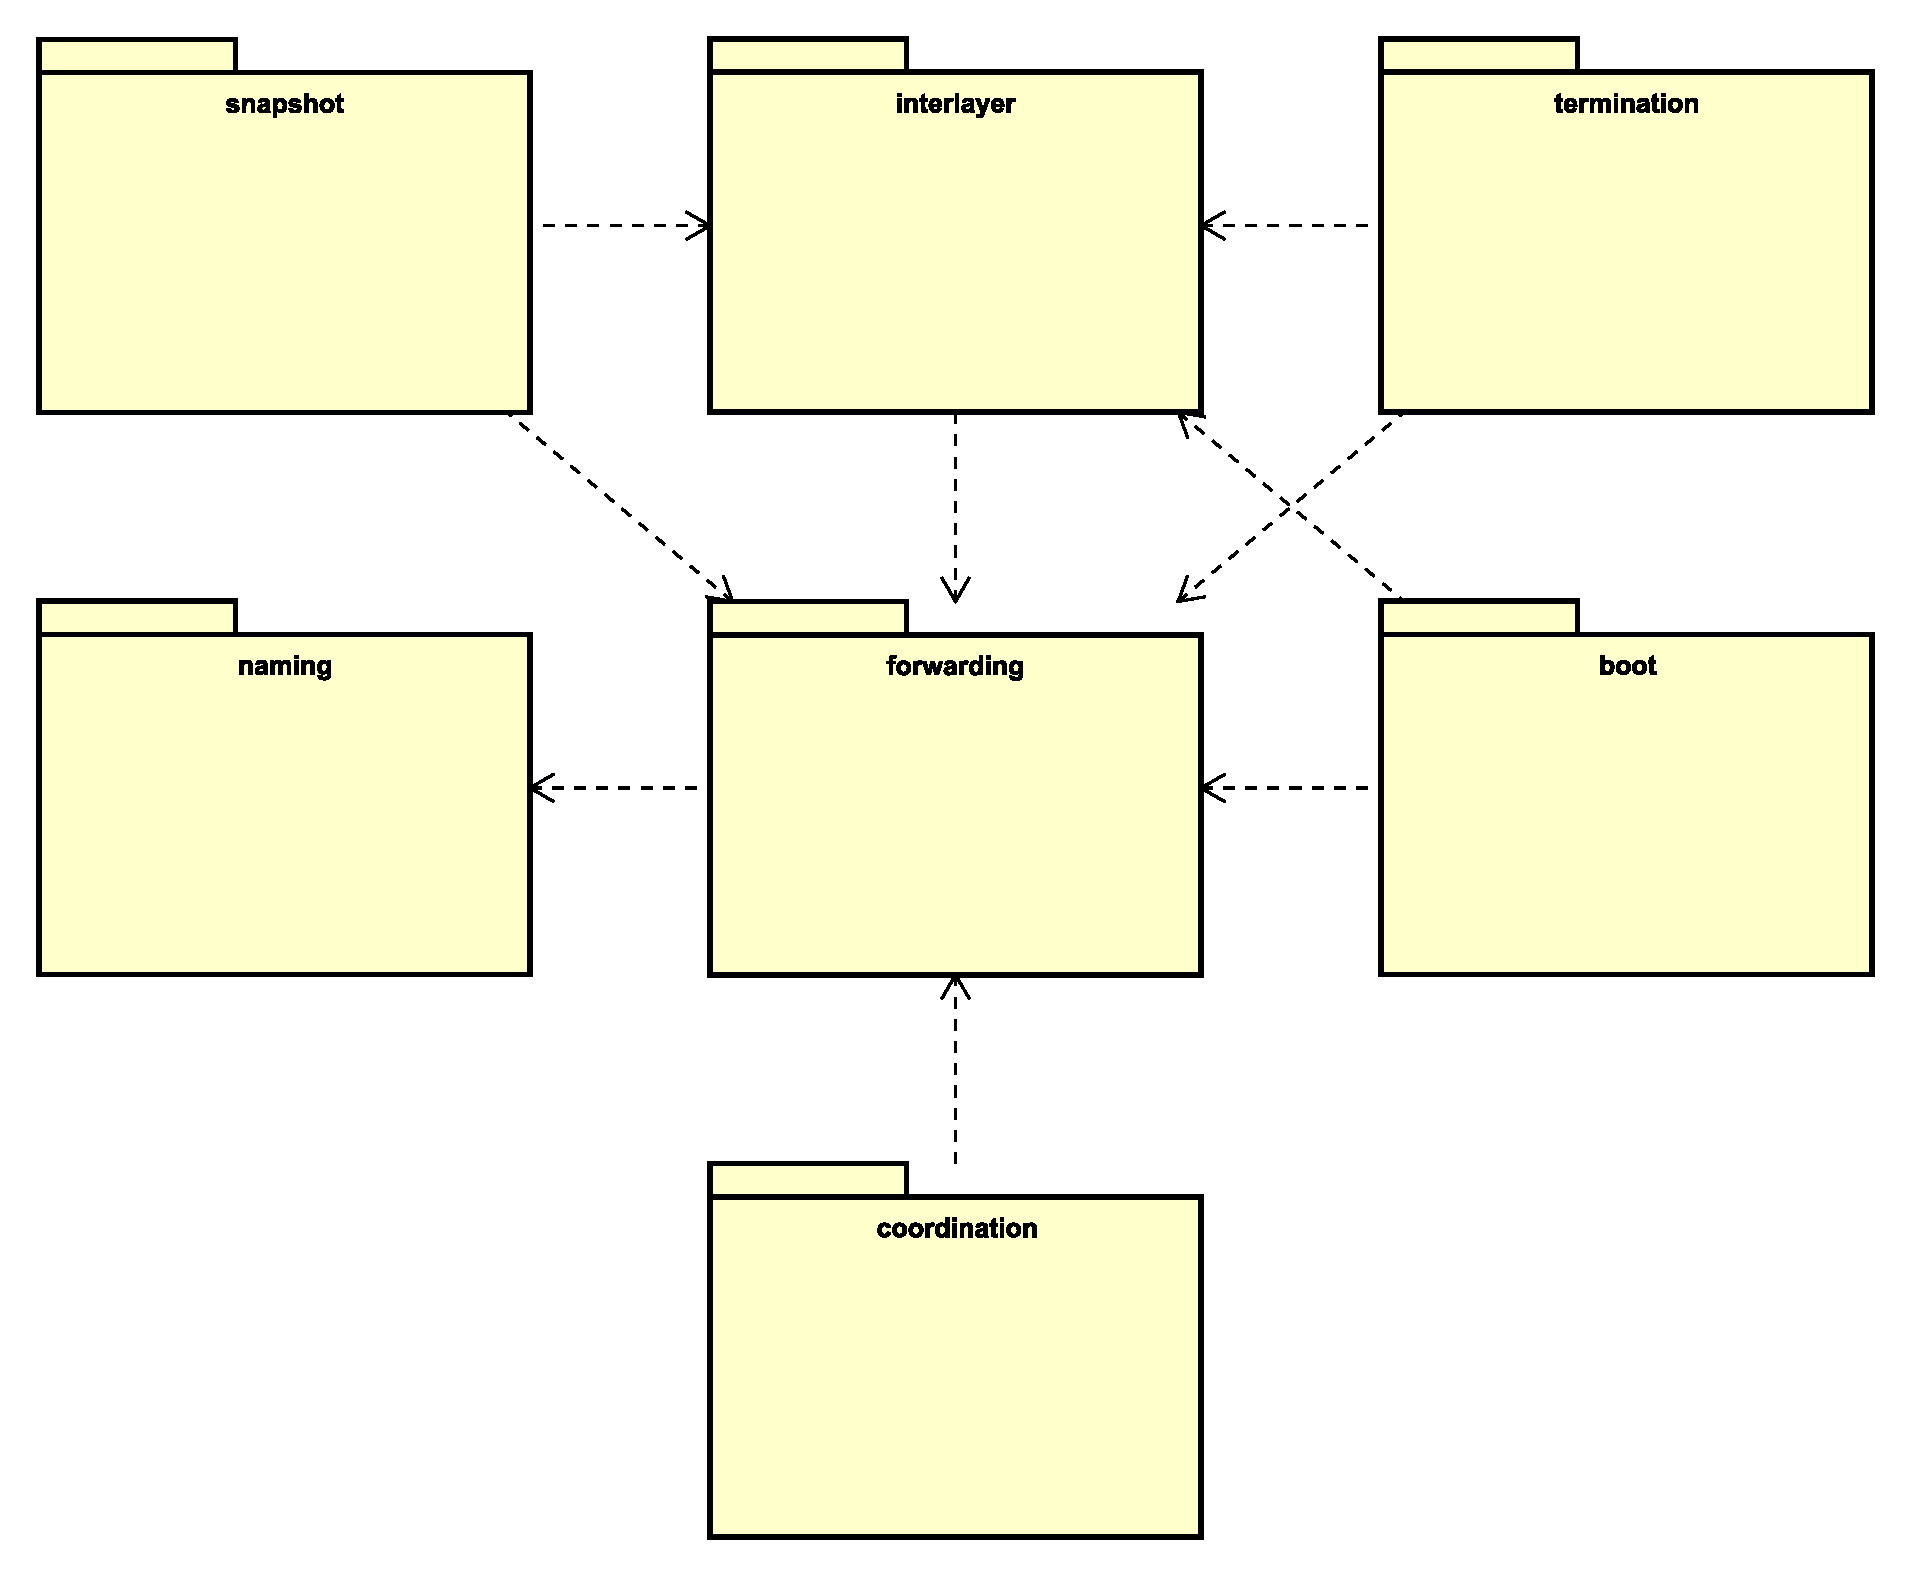
\includegraphics[height=9cm]{images/solution/mw/overview.eps}
  \caption{Middleware architecture overview}
  \label{fig:mw-arch-over}
\end{figure}

% \begin{itemize}
%   \item \texttt{naming}: service that provides a correspondence between logic
%     names and their actual location;
%   \item \texttt{forwarding}: service that represents the abstraction through
%     which it is possible to deliver messages to other middleware nodes;
%   \item \texttt{incoming}: service that is responsible of handling messages
%     coming from other middleware nodes;
%   \item \texttt{interlayer}: service that represents the interface between
%     the application and middleware layers;
%   \item \texttt{boot}: service that is responsible to start the system neatly;
%   \item \texttt{termination}: service that shut downs the node and the system
%     gracefully;
%   \item \texttt{snapshot}: service that takes consistent views of the node and
%     the system;
%   \item \texttt{coordination}: service that coordinates the interaction among
%     the nodes of the system;
%   \item \texttt{persistence}: service that provides a set of utilities to
%     store data in a persistent way.
% \end{itemize}

\subsubsubsection{Naming service}
The Naming service, fed with an reactive
entity id and its type, finds the node on
which a given reactive entity resides.

This is completely decoupled from the application
layer, which just provides the identifier and the type of the entity in the
headers of the message handed over to the middleware. Then, the
Naming component just have to look up for the node on which the reactive
entity resides through a local configuration file.

\subsubsubsection{Forwarding}
The Forwarding application delivers messages to other nodes. This component
comprise just an interface (\texttt{MQProxy}) and its
implementation (\texttt{RabbitSender}).

Basically, a \texttt{RabbitSender} takes a message as input and guarantees to
send it to the intended recipient, which could be middleware node or a
RabbitMQ pub/sub queue shared with the other message brokers.
\texttt{RabbitSender}s are able to make this decision by simply looking if the
messages they are handling are events or communications between districts.
In the former case, the messages are propagated towards the frontend of the
application (and therefore to the brokers). In the latter case, the messages are
sent to the district specified as the recipient of the message.

\subsubsubsection{Incoming}
The Incoming application is responsible of receiving messages from other
middleware nodes and to dispatch these messages to the appropriate middleware
application.
However, before dispatching this component process the message by applying some
checks: in fact, a message may be directed to another node or it might have to
be withheld if a snapshot is occurring.

Therefore, we decided to take advantage of Elixir's
\href{https://hexdocs.pm/gen_stage/GenStage.html}{GenStage} behaviour and
structure the modules of this component as a pipeline through which the
message is processed:

\begin{figure}[H]
  \centering
  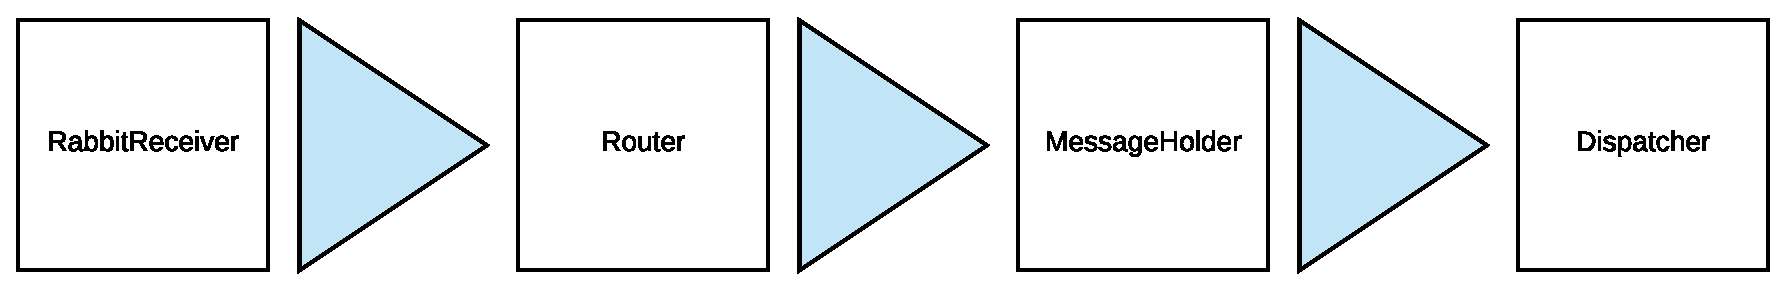
\includegraphics[width=\columnwidth]{images/solution/mw/inc/architect.eps}
  \caption{Incoming pipeline}
  \label{fig:mw-incoming}
\end{figure}

\begin{itemize}
  \item A RabbitReceiver is a process which receives messages from a single
    adjacent middleware node (or ``neighbor'') using RabbitMQ
  \item A Router compares the recipient field of the message with the
    identifier of the current node. If it is different, then it forwards the
    message to the next node along the path to the recipient
  \item A MessageHolder prevents messages to reach the dispatching point if a
    snapshot is happening. Then, when the snapshot ends, the messages will be
    forwarded again towards the Dispatcher
  \item A Dispatcher dispatches messages to a given application of the middleware
\end{itemize}

\begin{figure}[H]
  \centering
  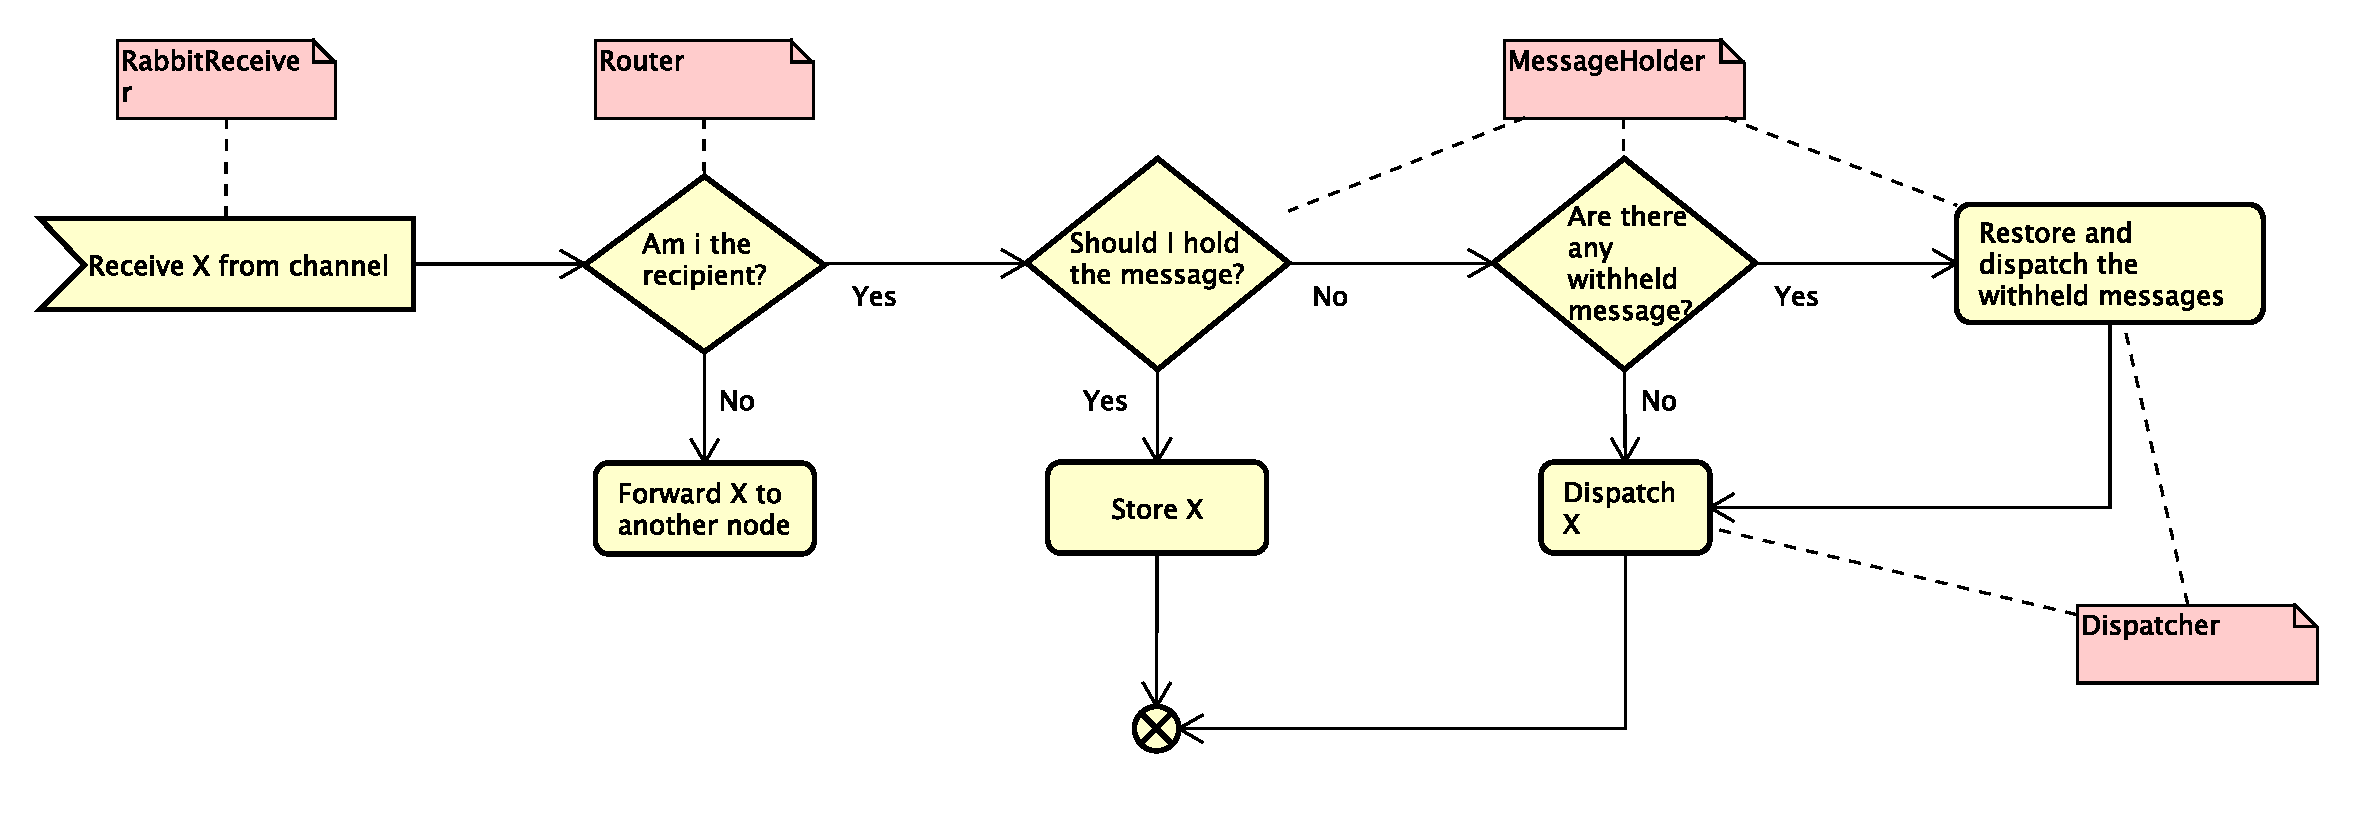
\includegraphics[width=\columnwidth]{images/solution/mw/inc/activity.eps}
  \caption{Activity diagram for Incoming pipeline}
  \label{fig:mw-incoming-activity}
\end{figure}

Thanks to the flexibility of GenStage, we can compose our pipelines by adding
an arbitrary number of elements at each stage of the pipeline. For instance,
there is one RabbitReceiver for each middleware neighbor plus one for loopback
communication: in this case, we just have to spawn as many RabbitReceivers as
needed and then make the Router subscribe to the events generated by them
(that is, the incoming messages).

\subsubsection{Interlayer service}

This component is responsible of the communication that is performed among
different layers, namely the one which it belongs (the \textbf{middleware}) and
another one who uses the middleware layer, that is the \textbf{application}
layer.

We show in figure \ref{fig:mw-interlayer} the architecture of this service and
then we will show in detail each module that composes this component.

\begin{figure}[H]
  \centering
  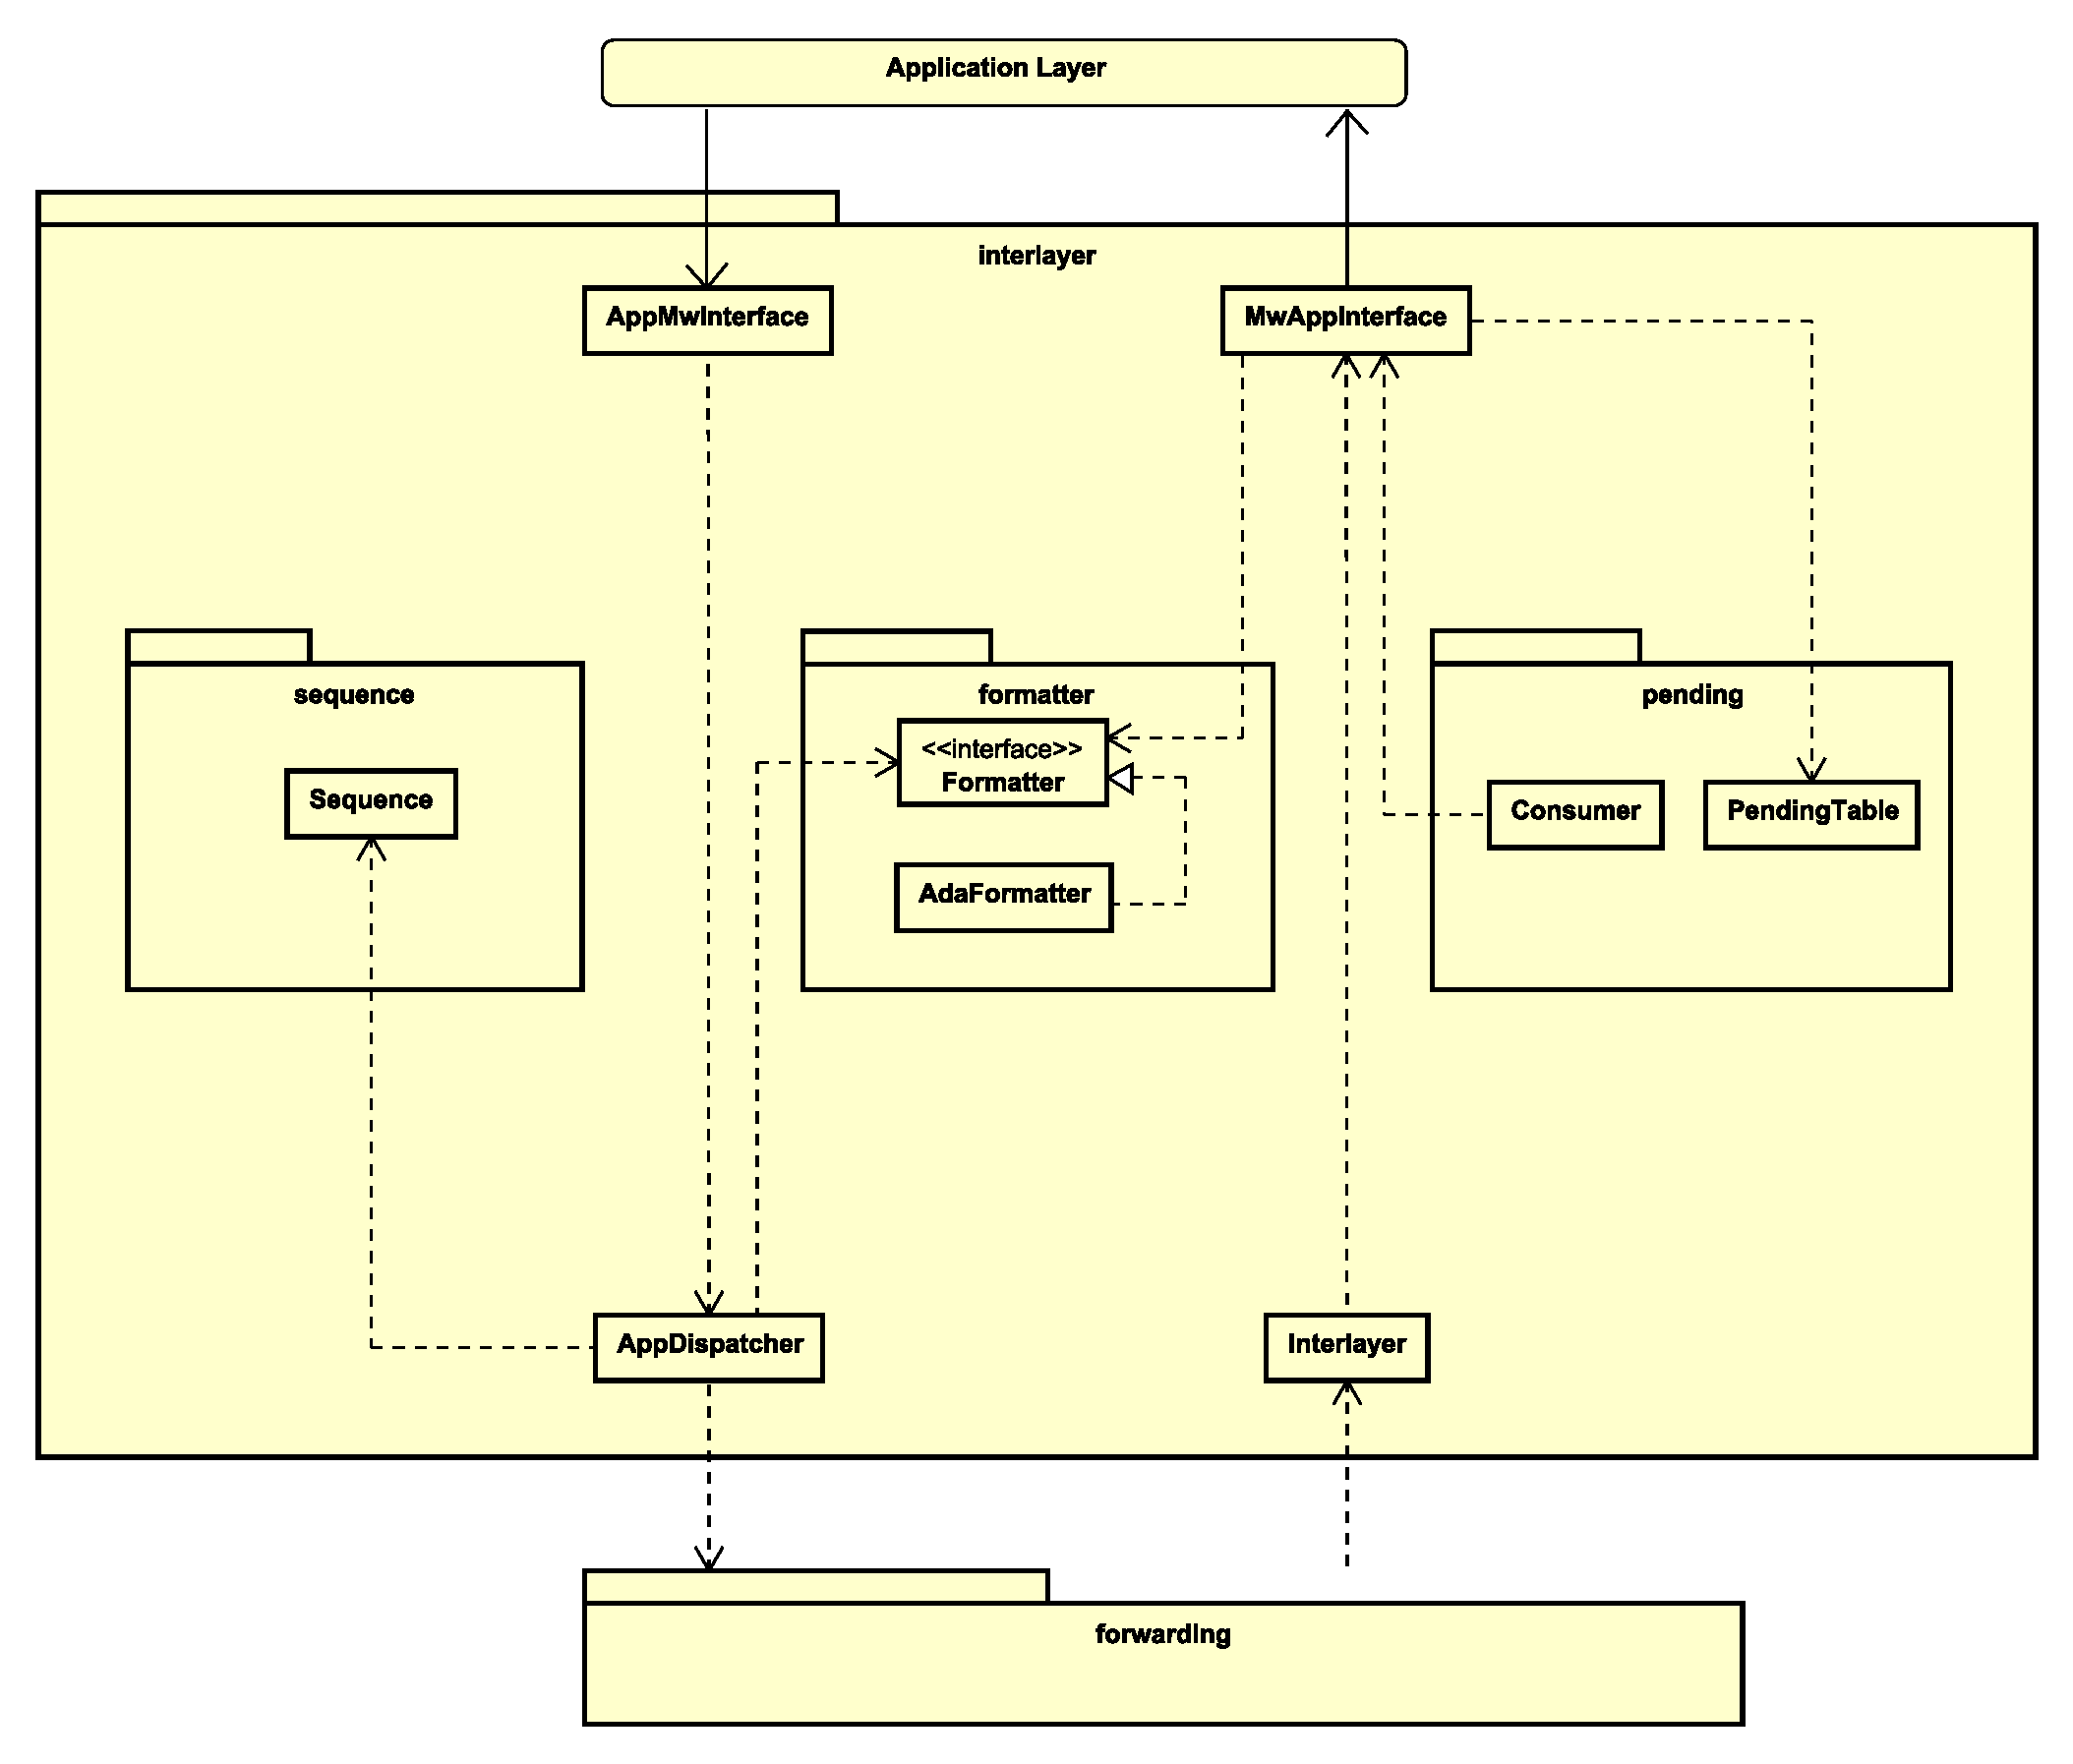
\includegraphics[width=\columnwidth]{images/solution/mw/interlayer.eps}
  \caption{Middleware's Interlayer service}
  \label{fig:mw-interlayer}
\end{figure} % TODO: needs update (Sequence usage comes from AppMwInterface)

% TODO: All class diagrams has to be added
\subsubsubsection{interlayer.Interlayer}

\subsubsubsection{interlayer.MwAppInterface}

\subsubsubsection{interlayer.AppMwInterface}

\subsubsubsection{interlayer.AppDispatcher}

\subsubsubsection{interlayer.sequence.Sequence}

\subsubsubsection{interlayer.formatter.Formatter}

\subsubsubsection{interlayer.formatter.AdaFormatter}

\subsubsubsection{interlayer.pending.PendingTable}

\subsubsubsection{interlayer.pending.Consumer}

\subsubsection{Boot service}\label{sec:mw-boot-descr}

The Boot service is responsible of starting the system in a graceful fashion.
It does so by dividing the start phase into two subphases, namely the
\textbf{marker diffusion} and the \textbf{(own) boot} phase. The procedure is
the same shown in Figure \ref{fig:sys-bootstrap-protocol}, with the first phase
going from left to right and the second phase going in the opposite direction.

In this context, by \textit{marker} we will mean \textit{boot marker}.

When receiving a marker, this the Boot service will forward the marker to all
of its adjacent middleware nodes.
Then, when receiving further markers, this service will just reply immediately
with an end marker.

After having received all the replies for the markers, the Boot service will
request to the application layer to gracefully start.
When the application layer will inform the middleware it started, this service
will send an end marker to all of its adjacent middleware nodes.

\subsubsubsection{Termination service}\label{sec:mw-termination-descr}

The Termination service is responsible of shutting down the system in a
graceful fashion.
It does so by dividing the termination phase into two subphases, namely the
\textbf{marker diffusion} and the \textbf{(own) termination} phase. The
procedure is the same shown in Figure \ref{fig:sys-termination-protocol}, with
the first phase going from left to right and the second phase going in the
opposite direction.

In this context, by \textit{marker} we will mean \textit{termination marker}.

When receiving a marker, this the Termination service will forward the marker
to all of its adjacent middleware nodes.
Then, when receiving further markers, this service will just reply immediately
with an end marker.

After having received all the replies for the markers, the Termination service
will request to the application layer to gracefully shut down.
When the application layer will inform the middleware it has terminated, this
service will send an end marker to all of its adjacent middleware nodes.

\subsubsection{Snapshot service}
This component is responsible of taking snapshots.

We show in figure \ref{fig:mw-snapshot} the architecture of this service and
then we will show in detail each module that composes this component.

\begin{figure}[H]
  \centering
  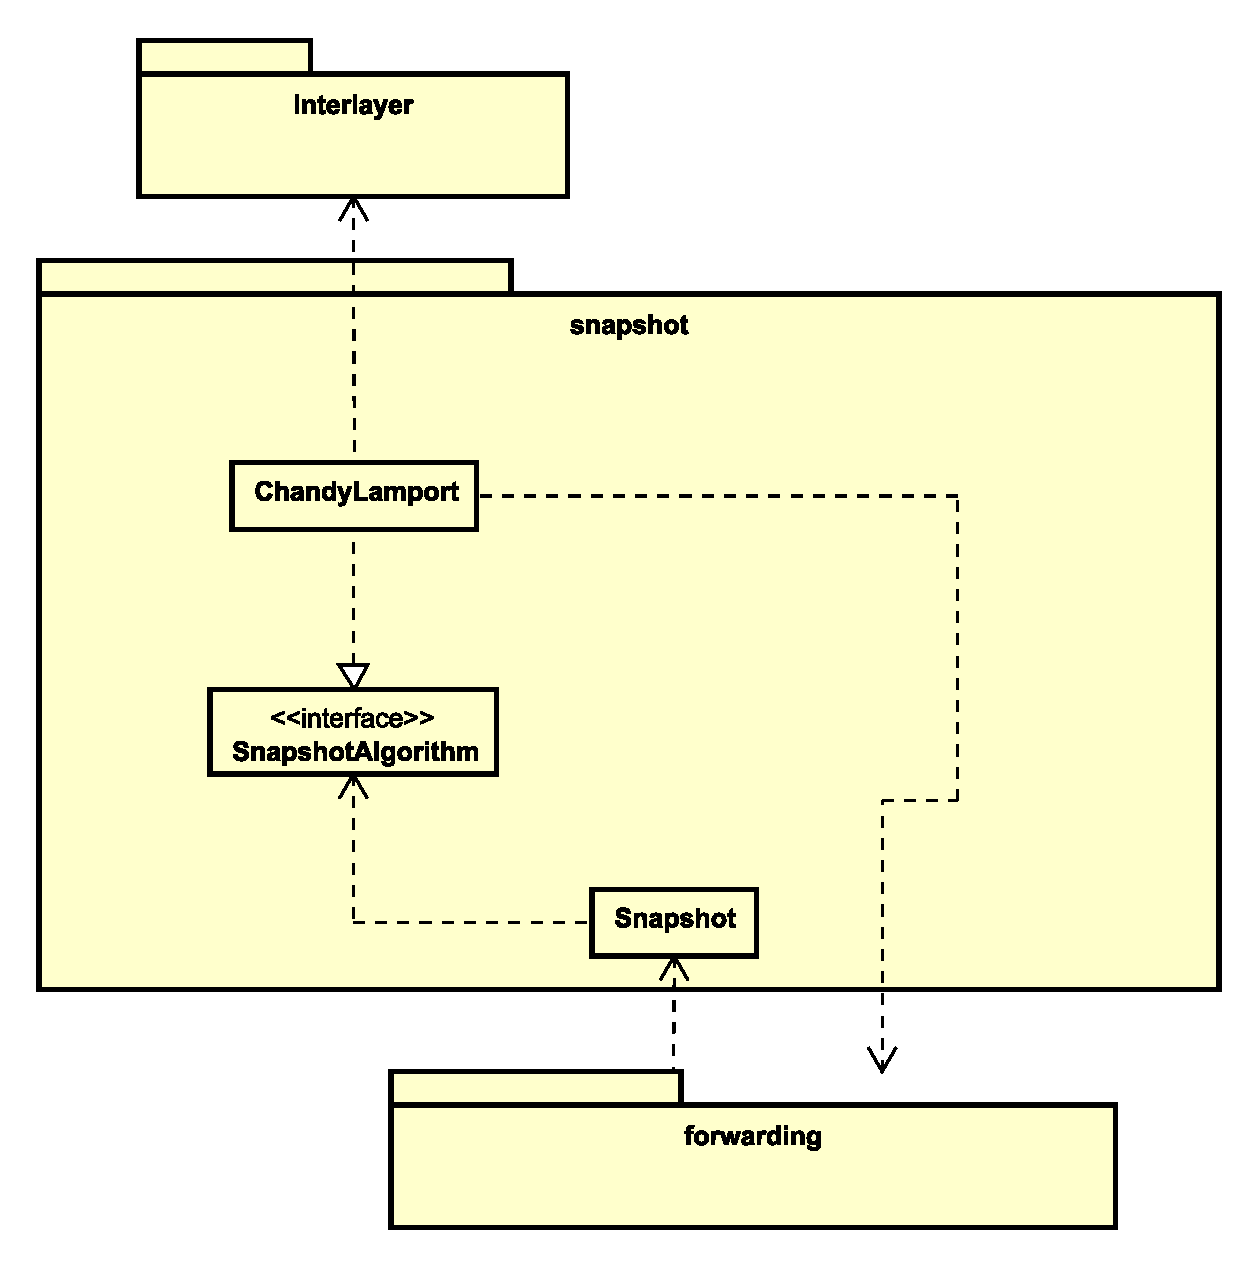
\includegraphics[width=\columnwidth]{images/solution/mw/snapshot.eps}
  \caption{Middleware's Snapshot service}
  \label{fig:mw-snapshot}
\end{figure}

% TODO: All class diagrams have to be added
\subsubsubsection{snapshot.Snapshot}
% TODO: Class diagram
\FloatBarrier
\begin{itemize}
  \item \textbf{Description} \\
    This module is the Fa\c cade of the Snapshot service. It is responsible
    to boot neatly and supervise all processes in Snapshot. Also, it has to
    handle snapshot requests that come from other nodes of the system.
  \item \textbf{Attributes}
  \item \textbf{Operations}
  \begin{itemize}
    \item \texttt{+ start()} \\
    Starts the Snapshot service.
    \item \texttt{+ handleMessage(message: String)} \\
    % TODO: check this out: Message will really be a String?
    Handles a snapshot start/termination request that comes from other nodes
    or receives snapshot information from the application layer.
  \end{itemize}
\end{itemize}

\subsubsubsection{snapshot.SnapshotAlgorithm}
% TODO: Class diagram
\FloatBarrier
\begin{itemize}
  \item \textbf{Description} \\
    Interface for processes that implement a certain kind of snapshot.
  \item \textbf{Attributes}
  \item \textbf{Operations}
  \begin{itemize}
    \item \texttt{+ take()} \\
    Starts to take a snapshot.
    \item \texttt{+ submitLocalSnapshot()} \\
    Stores a local snapshot.
    \item \texttt{+ submitRemoteSnapshot()} \\
    Stores a remote snapshot.
  \end{itemize}
\end{itemize}

\subsubsubsection{snapshot.ChandyLamport}
% TODO: Class diagram
\FloatBarrier
\begin{itemize}
  \item \textbf{Description} \\
    Module that implements the \texttt{snapshot.SnapshotAlgorithm}
    interface to take snapshots with the algorithm by Chandy and Lamport.
  \item \textbf{Attributes}
  \item \textbf{Operations}
  \begin{itemize}
    \item \texttt{+ take()} \\
    Starts to take a snapshot: that implies Forwarding module to notify
    other nodes of that and to hold messages until the snapshot is over; also
    that implies Interlayer to issue a snapshot request to the application
    layer.
    \item \texttt{+ submitLocalSnapshot()} \\
    Stores the snapshot of the node where the process is executing.
    \item \texttt{+ submitRemoteSnapshot()} \\
    Stores the snapshot of a remote node.
  \end{itemize}
\end{itemize}

\subsubsubsection{Coordination}

This component is responsible of the supervising the life-cycle of an
application run on our middleware, so our backend is able to operate
cohesively.

There are just two architectural units which compose this service:

\begin{enumerate}
\item a \texttt{Coordinator} initiates the boot process when requested and the
  termination process when the time limit for the application elapses;
\item \texttt{Monitor}s supervise the status of some services. In
  particular, we instantiated two monitor processes, one for the boot process
  and another one for the termination process. If a process $X$ does not end
  within a pre-configured time limit (we arbitrarily set 15 seconds for this
  parameter) after being started, the monitor issues again a request to
  perform $X$.
\end{enumerate}

\subsubsubsection{Persistence}

This component is an adapter towards persistence and caching applications.

More specifically, persistence is a collection of Redix wrappers. Redix is an
Elixir client for Redis, which handles all the network communication and
provides simple and convenient API to access Redis applications.
Therefore, we just have to specify some of the CRUD operations for a certain
data structure we are interested in: it could be a map (e.g., for pending
requests, so that we are able to correlate an id to a given request) or a
queue (e.g., pending unsent messages directed to the application layer).

However, we stress the fact that even if Persistence application uses Redis, it
could have used anything else without changing its API (the persistence
technology we employed is completely transparent to the other middleware
applications).

